\section{Base de Datos}

Utilizando PostgreSQL como gestor de bases de datos, se diseña sobre este la base de datos \texttt{\textbf{"BaseDePatos"}} que servirá para almacenar y gestionar la información de productos y servicios. Sin embargo, previo a la generación del sistema es importante definir aspectos fundamnetales como el los modelos de caso de uso, la definición estructural de las tablas, etc. Algunos de estos aspectos se detallan a continuación:

\subsection{Modelo Entidad Relación Físico}

Es el modelo que representa la estructura física de la base de datos, incluyendo las tablas, sus atributos, tipos de datos, claves primarias y foráneas, así como las relaciones entre ellas. Este modelo se basa en el modelo lógico y se ajusta a las características específicas del sistema de gestión de productos y servicios.

\begin{figure}[H]
  \centering
  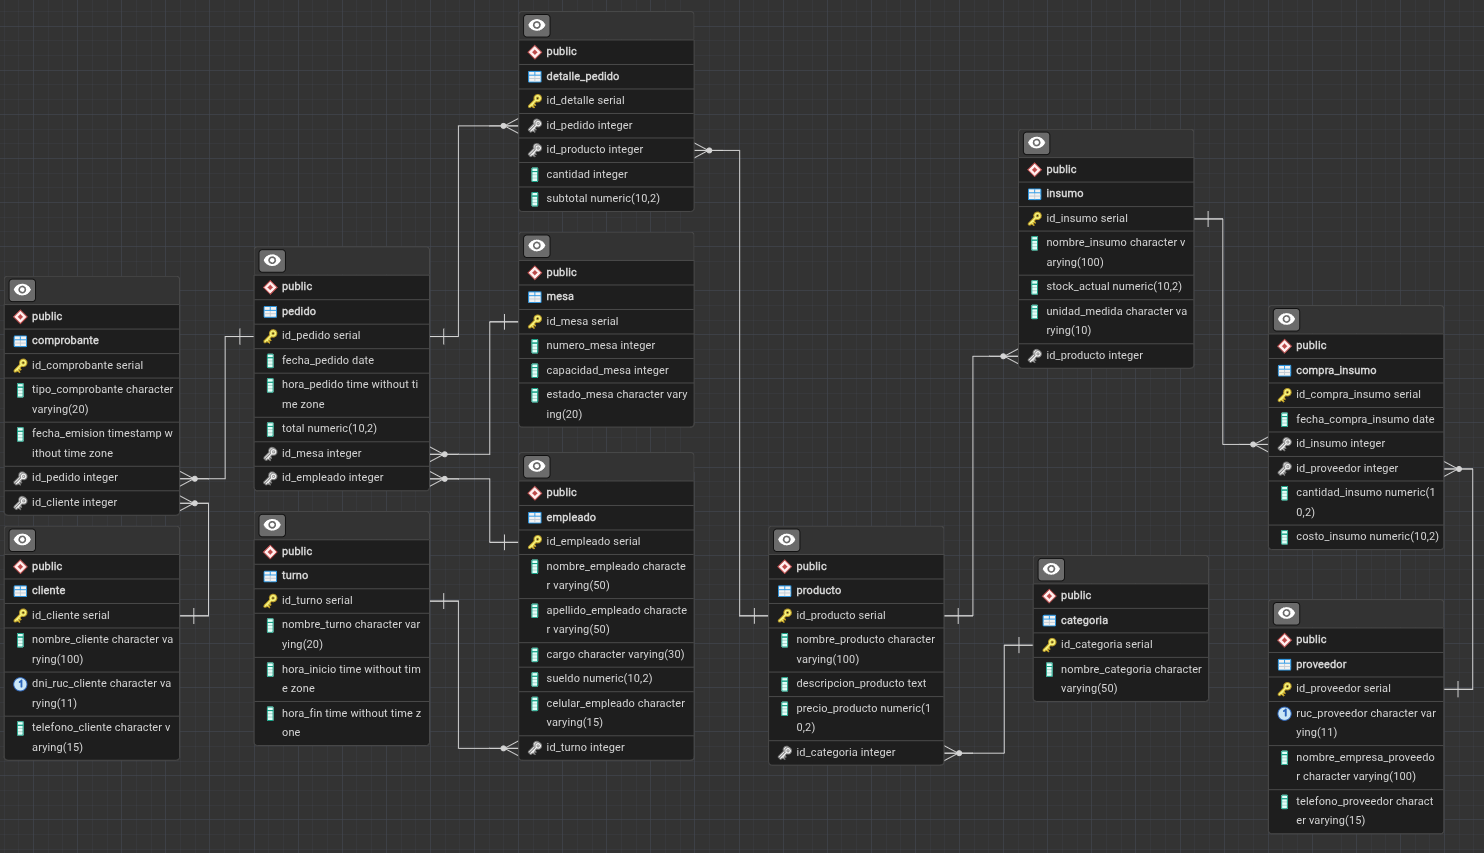
\includegraphics[width=1\textwidth]{./assets/MER-fisico.png}
  \caption{Modelo Entidad Relación Físico}
\end{figure}

\subsection{Modelo Entidad Relación Lógico}

Es el modelo que representa la estructura lógica de la base de datos, incluyendo las entidades, sus atributos, claves primarias y foráneas, así como las relaciones entre ellas. Este modelo se basa en el modelo conceptual y se ajusta a las necesidades del sistema de gestión de productos y servicios.

\begin{figure}[H]
  \centering
  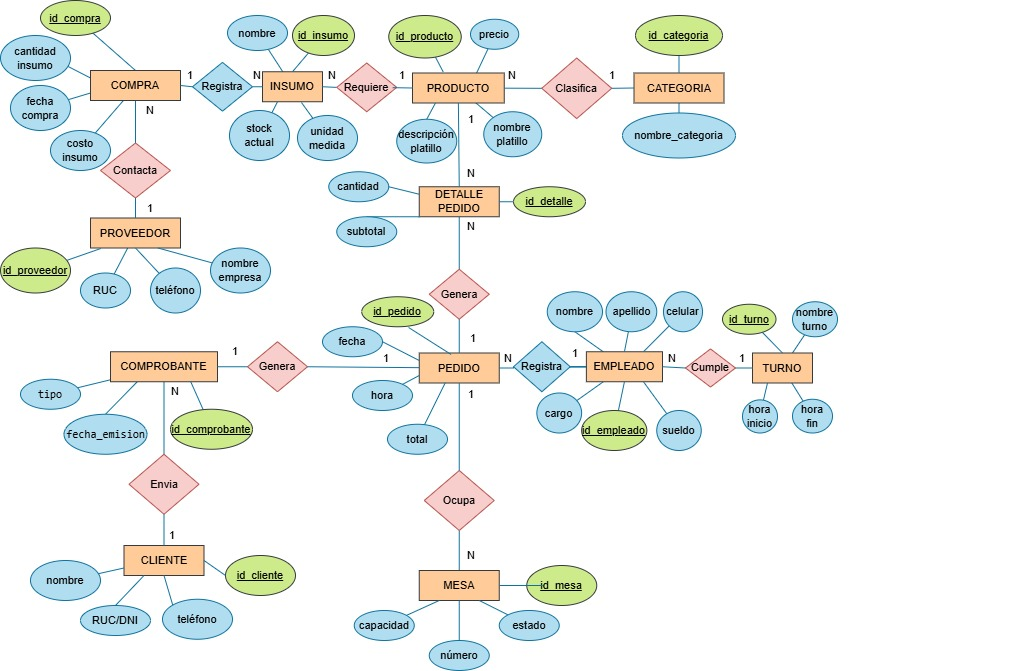
\includegraphics[width=1\textwidth]{./assets/der_logico.jpeg}
  \caption{Modelo Entidad Relación Lógico}
\end{figure}

Este modelo lógico se ha diseñado para reflejar las necesidades del sistema de gestión de productos y servicios, permitiendo una estructura clara y eficiente para almacenar y gestionar la información relacionada con los productos, servicios, clientes, pedidos, etc.

Es importante destacar que el modelo lógico es una representación abstracta de la base de datos, y su diseño se basa en los requisitos del sistema y las mejores prácticas de modelado de datos. Así mismo, el modelo físico se ajusta a las características específicas del sistema y del gestor de bases de datos utilizado mientras que el lógico se centra en la estructura lógica de los datos y las relaciones entre ellos, sin preocuparse por los detalles de implementación específicos del gestor de bases de datos.

\newpage

\subsection{Modelo de Caso de Uso}

Son representaciones gráficas que describen las interacciones entre los usuarios (actores) y los procesos del sistema. Estos modelos ayudan a identificar los requisitos funcionales del sistema y a diseñar la base de datos de manera que soporte adecuadamente las funcionalidades requeridas.

A continuación se presenta el modelo de caso de uso general:

\begin{figure}[H]
  \centering
  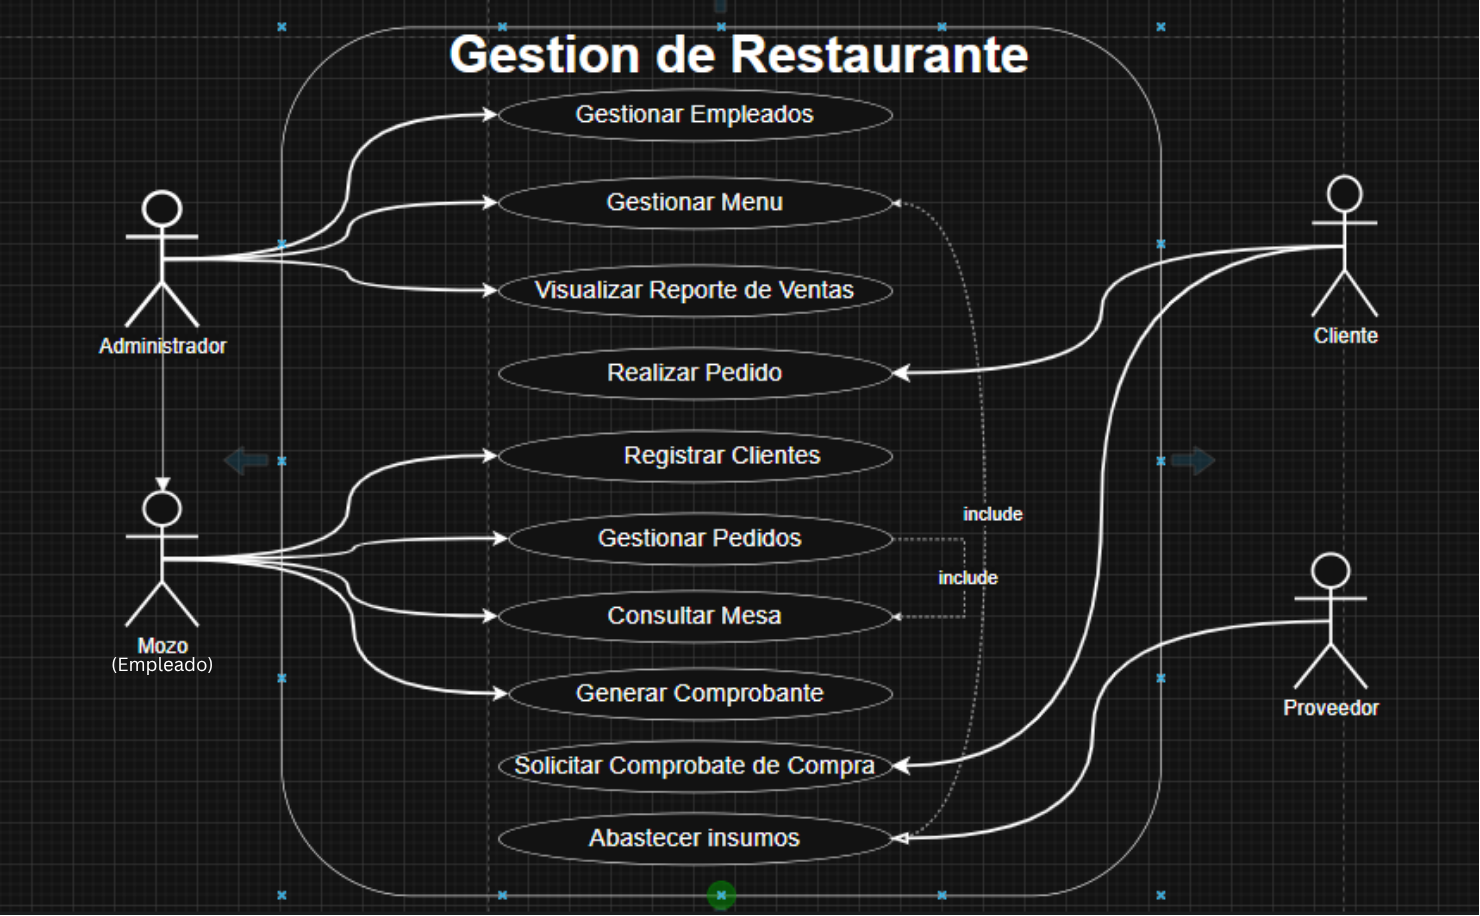
\includegraphics[width=1\textwidth]{./assets/modelo_caso_de_uso.png}
  \caption{Modelo de Caso de Uso General}
\end{figure}

En este modelo de caso de uso general, se identifican los actores principales que interactúan con el sistema, como el cliente, el administrador y el sistema de gestión de productos y servicios. Cada actor tiene diferentes casos de uso asociados, que representan las funcionalidades específicas que pueden realizar dentro del sistema.

\newpage

\subsection{Diagramas de Flujo}

Los diagramas de flujo representan visualmente el flujo que cada proceso presente dentro del diagrama de caso de uso general, permitiendo entender cómo se llevan a cabo las diferentes tareas y cómo interactúan entre sí. A continuación se presentan algunos diagramas de flujo para procesos específicos:

\subsubsection{Gestión de Pagos}

Este diagrama de flujo representa el proceso de gestión de pagos dentro del sistema, mostrando las diferentes etapas que se llevan a cabo para procesar un pago, desde la selección del método de pago hasta la confirmación del pago y la actualización del estado del pedido.

\begin{figure}[H]
  \centering
  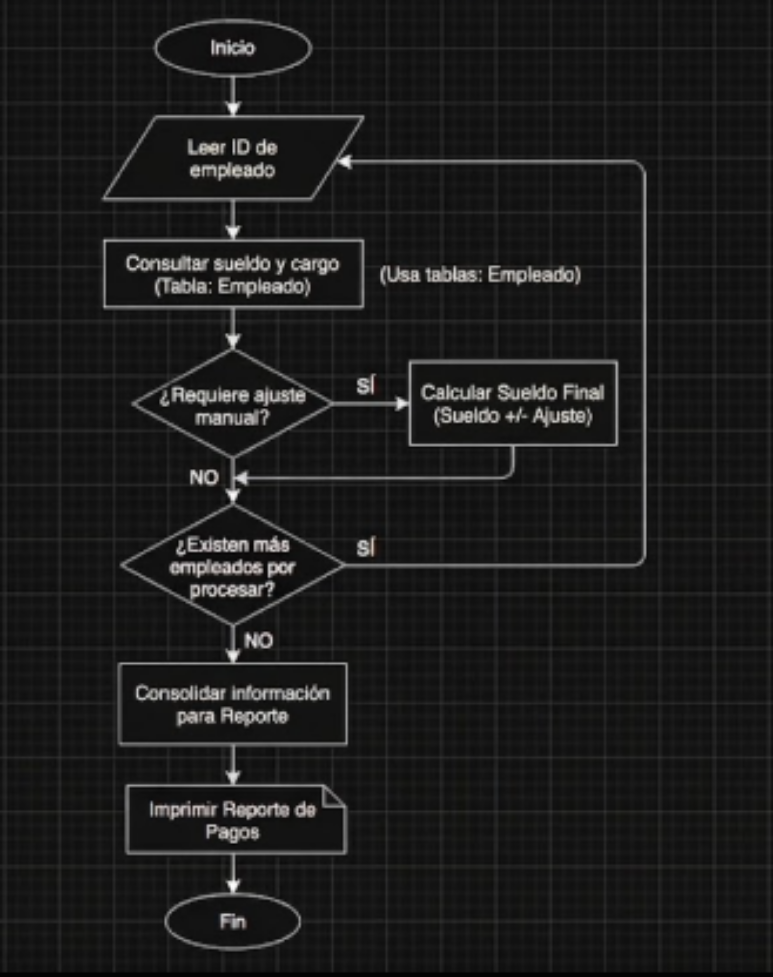
\includegraphics[width=0.8\textwidth]{./assets/flujo_gestionar_pagos.png}
  \caption{Diagrama de Flujo para el Proceso de Gestión de Pagos}
\end{figure}


\subsection{Creación de la Base de Datos y Tablas}

A continuación se presentan las evidencias de la creación y población de la base de datos utilizando PostgreSQL:

\begin{itemize}
  \item \textbf{Creación de la Base de Datos:}
  \begin{figure}[H]
    \centering
    
\includegraphics[width=0.8\textwidth]{./assets/c1.png}
    \caption{Evidencia de la creación de la base de datos \texttt{"BaseDePatos"} en terminal mediante psql.}
  \end{figure}
  \item \textbf{Moviéndose a la base de datos:}
  \begin{figure}[H]
    \centering
    
\includegraphics[width=0.8\textwidth]{./assets/c2.png}
    \caption{Evidencia de la selección de la base de datos \texttt{"BaseDePatos"} en terminal mediante psql.}
  \end{figure}
  \item \textbf{Categorías:}
    \begin{listing}[H]
        \centering
        \begin{minted}[
            frame=lines,
            linenos,
            breaklines,
            fontsize=\footnotesize,
            numbersep=5pt,  % espacio entre números y código
            xleftmargin=20pt,  % margen izquierdo extra para los números
            tabsize=4
        ]{sql}
        CREATE TABLE public.categoria (
            id_categoria serial4 NOT NULL,
            nombre_categoria varchar(50) NOT NULL,
            CONSTRAINT categoria_pkey PRIMARY KEY (id_categoria)
        );
        \end{minted}
        \caption{Fragmento de código SQL para la creación de la tabla \texttt{categoria}.}
        \label{lst:categoria}
    \end{listing}
  \item \textbf{Cliente}
    \begin{listing}[H]
        \centering
        \begin{minted}[
            frame=lines,
            linenos,
            breaklines,
            fontsize=\footnotesize,
            numbersep=5pt,  % espacio entre números y código
            xleftmargin=20pt,  % margen izquierdo extra para los números
            tabsize=4
        ]{sql}
        CREATE TABLE public.cliente (
          id_cliente serial4 NOT NULL,
          nombre_cliente varchar(100) NOT NULL,
          dni_ruc_cliente varchar(11) NULL,
          telefono_cliente varchar(15) NULL,
          CONSTRAINT cliente_dni_ruc_cliente_key UNIQUE (dni_ruc_cliente),
          CONSTRAINT cliente_pkey PRIMARY KEY (id_cliente)
        );
        \end{minted}
        \caption{Fragmento de código SQL para la creación de la tabla \texttt{cliente}.}
        \label{lst:cliente}
    \end{listing}
    \newpage
    \item \textbf{Mesa}
%     CREATE TABLE public.mesa (
%     id_mesa serial4 NOT NULL,
%     numero_mesa int4 NOT NULL,
%     capacidad_mesa int4 NULL,
%     estado_mesa varchar(20) DEFAULT 'Libre'::character varying NULL,
%     CONSTRAINT mesa_pkey PRIMARY KEY (id_mesa)
% );
    \begin{listing}[H]
        \centering
        \begin{minted}[
            frame=lines,
            linenos,
            breaklines,
            fontsize=\footnotesize,
            numbersep=5pt,  % espacio entre números y código
            xleftmargin=20pt,  % margen izquierdo extra para los números
            tabsize=4
        ]{sql}
        CREATE TABLE public.mesa (
          id_mesa serial4 NOT NULL,
          numero_mesa int4 NOT NULL,
          capacidad_mesa int4 NULL,
          estado_mesa varchar(20) DEFAULT 'Libre'::character varying NULL,
          CONSTRAINT mesa_pkey PRIMARY KEY (id_mesa)
        );
        \end{minted}
        \caption{Fragmento de código SQL para la creación de la tabla \texttt{mesa}.}
        \label{lst:mesa}
    \end{listing}
    \newpage
    \item \textbf{Proveedor}
%     CREATE TABLE public.proveedor (
%     id_proveedor serial4 NOT NULL,
%     ruc_proveedor varchar(11) NOT NULL,
%     nombre_empresa_proveedor varchar(100) NOT NULL,
%     telefono_proveedor varchar(15) NULL,
%     CONSTRAINT proveedor_pkey PRIMARY KEY (id_proveedor),
%     CONSTRAINT proveedor_ruc_proveedor_key UNIQUE (ruc_proveedor)
% );
    \begin{listing}[H]
        \centering
        \begin{minted}[
            frame=lines,
            linenos,
            breaklines,
            fontsize=\footnotesize,
            numbersep=5pt,  % espacio entre números y código
            xleftmargin=20pt,  % margen izquierdo extra para los números
            tabsize=4
        ]{sql}
        CREATE TABLE public.proveedor (
          id_proveedor serial4 NOT NULL,
          ruc_proveedor varchar(11) NOT NULL,
          nombre_empresa_proveedor varchar(100) NOT NULL,
          telefono_proveedor varchar(15) NULL,
          CONSTRAINT proveedor_pkey PRIMARY KEY (id_proveedor),
          CONSTRAINT proveedor_ruc_proveedor_key UNIQUE (ruc_proveedor)
        );
        \end{minted}
        \caption{Fragmento de código SQL para la creación de la tabla \texttt{proveedor}.}
        \label{lst:proveedor}
    \end{listing}
    \item \textbf{Turno}
%     CREATE TABLE public.turno (
%     id_turno serial4 NOT NULL,
%     nombre_turno varchar(20) NOT NULL,
%     hora_inicio time NULL,
%     hora_fin time NULL,
%     CONSTRAINT turno_pkey PRIMARY KEY (id_turno)
% );
    \begin{listing}[H]
        \centering
        \begin{minted}[
            frame=lines,
            linenos,
            breaklines,
            fontsize=\footnotesize,
            numbersep=5pt,  % espacio entre números y código
            xleftmargin=20pt,  % margen izquierdo extra para los números
            tabsize=4
        ]{sql}
        CREATE TABLE public.turno (
          id_turno serial4 NOT NULL,
          nombre_turno varchar(20) NOT NULL,
          hora_inicio time NULL,
          hora_fin time NULL,
          CONSTRAINT turno_pkey PRIMARY KEY (id_turno)
        );
        \end{minted}
        \caption{Fragmento de código SQL para la creación de la tabla \texttt{turno}.}
        \label{lst:turno}
    \end{listing}
    \item \textbf{Empleado}
%   CREATE TABLE public.empleado (
%     id_empleado serial4 NOT NULL,
%     nombre_empleado varchar(50) NOT NULL,
%     apellido_empleado varchar(50) NOT NULL,
%     cargo varchar(30) NULL,
%     sueldo numeric(10, 2) NULL,
%     celular_empleado varchar(15) NULL,
%     id_turno int4 NULL,
%     CONSTRAINT empleado_pkey PRIMARY KEY (id_empleado),
%     CONSTRAINT fk_empleado_turno FOREIGN KEY (id_turno) REFERENCES public.turno(id_turno)
% );
    \begin{listing}[H]
        \centering
        \begin{minted}[
            frame=lines,
            linenos,
            breaklines,
            fontsize=\footnotesize,
            numbersep=5pt,  % espacio entre números y código
            xleftmargin=20pt,  % margen izquierdo extra para los números
            tabsize=4
        ]{sql}
        CREATE TABLE public.empleado (
          id_empleado serial4 NOT NULL,
          nombre_empleado varchar(50) NOT NULL,
          apellido_empleado varchar(50) NOT NULL,
          cargo varchar(30) NULL,
          sueldo numeric(10, 2) NULL,
          celular_empleado varchar(15) NULL,
          id_turno int4 NULL,
          CONSTRAINT empleado_pkey PRIMARY KEY (id_empleado),
          CONSTRAINT fk_empleado_turno FOREIGN KEY (id_turno) REFERENCES public.turno(id_turno)
        );
        \end{minted}
        \caption{Fragmento de código SQL para la creación de la tabla \texttt{empleado}.}
        \label{lst:empleado}
    \end{listing}
    \newpage
    \item \textbf{Pedido}
%     CREATE TABLE public.pedido (
%     id_pedido serial4 NOT NULL,
%     fecha_pedido date DEFAULT CURRENT_DATE NULL,
%     hora_pedido time DEFAULT CURRENT_TIME NULL,
%     total numeric(10, 2) DEFAULT 0 NULL,
%     id_mesa int4 NULL,
%     id_empleado int4 NULL,
%     CONSTRAINT pedido_pkey PRIMARY KEY (id_pedido),
%     CONSTRAINT pedido_id_empleado_fkey FOREIGN KEY (id_empleado) REFERENCES public.empleado(id_empleado),
%     CONSTRAINT pedido_id_mesa_fkey FOREIGN KEY (id_mesa) REFERENCES public.mesa(id_mesa)
% );
    \begin{listing}[H]
        \centering
        \begin{minted}[
            frame=lines,
            linenos,
            breaklines,
            fontsize=\footnotesize,
            numbersep=5pt,  % espacio entre números y código
            xleftmargin=20pt,  % margen izquierdo extra para los números
            tabsize=4
        ]{sql}
        CREATE TABLE public.pedido (
          id_pedido serial4 NOT NULL,
          fecha_pedido date DEFAULT CURRENT_DATE NULL,
          hora_pedido time DEFAULT CURRENT_TIME NULL,
          total numeric(10, 2) DEFAULT 0 NULL,
          id_mesa int4 NULL,
          id_empleado int4 NULL,
          CONSTRAINT pedido_pkey PRIMARY KEY (id_pedido),
          CONSTRAINT pedido_id_empleado_fkey FOREIGN KEY (id_empleado) REFERENCES public.empleado(id_empleado),
          CONSTRAINT pedido_id_mesa_fkey FOREIGN KEY (id_mesa) REFERENCES public.mesa(id_mesa)
        );
        \end{minted}
        \caption{Fragmento de código SQL para la creación de la tabla \texttt{pedido}.}
        \label{lst:pedido}
    \end{listing}
    \item \textbf{Producto}
%     CREATE TABLE public.producto (
%     id_producto serial4 NOT NULL,
%     nombre_producto varchar(100) NOT NULL,
%     descripcion_producto text NULL,
%     precio_producto numeric(10, 2) NOT NULL,
%     id_categoria int4 NULL,
%     CONSTRAINT producto_pkey PRIMARY KEY (id_producto),
%     CONSTRAINT producto_id_categoria_fkey FOREIGN KEY (id_categoria) REFERENCES public.categoria(id_categoria)
% );
    \begin{listing}[H]
        \centering
        \begin{minted}[
            frame=lines,
            linenos,
            breaklines,
            fontsize=\footnotesize,
            numbersep=5pt,  % espacio entre números y código
            xleftmargin=20pt,  % margen izquierdo extra para los números
            tabsize=4
        ]{sql}
        CREATE TABLE public.producto (
          id_producto serial4 NOT NULL,
          nombre_producto varchar(100) NOT NULL,
          descripcion_producto text NULL,
          precio_producto numeric(10, 2) NOT NULL,
          id_categoria int4 NULL,
          CONSTRAINT producto_pkey PRIMARY KEY (id_producto),
          CONSTRAINT producto_id_categoria_fkey FOREIGN KEY (id_categoria) REFERENCES public.categoria(id_categoria)
        );
        \end{minted}
        \caption{Fragmento de código SQL para la creación de la tabla \texttt{producto}.}
        \label{lst:producto}
    \end{listing}
      \item \textbf{Comprobante}
%       CREATE TABLE public.comprobante (
%     id_comprobante serial4 NOT NULL,
%     tipo_comprobante varchar(20) NULL,
%     fecha_emision timestamp DEFAULT CURRENT_TIMESTAMP NULL,
%     id_pedido int4 NULL,
%     id_cliente int4 NULL,
%     CONSTRAINT comprobante_pkey PRIMARY KEY (id_comprobante),
%     CONSTRAINT comprobante_id_cliente_fkey FOREIGN KEY (id_cliente) REFERENCES public.cliente(id_cliente),
%     CONSTRAINT comprobante_id_pedido_fkey FOREIGN KEY (id_pedido) REFERENCES public.pedido(id_pedido)
% );
    \begin{listing}[H]
        \centering
        \begin{minted}[
            frame=lines,
            linenos,
            breaklines,
            fontsize=\footnotesize,
            numbersep=5pt,  % espacio entre números y código
            xleftmargin=20pt,  % margen izquierdo extra para los números
            tabsize=4
        ]{sql}
        CREATE TABLE public.comprobante (
          id_comprobante serial4 NOT NULL,
          tipo_comprobante varchar(20) NULL,
          fecha_emision timestamp DEFAULT CURRENT_TIMESTAMP NULL,
          id_pedido int4 NULL,
          id_cliente int4 NULL,
          CONSTRAINT comprobante_pkey PRIMARY KEY (id_comprobante),
          CONSTRAINT comprobante_id_cliente_fkey FOREIGN KEY (id_cliente) REFERENCES public.cliente(id_cliente),
          CONSTRAINT comprobante_id_pedido_fkey FOREIGN KEY (id_pedido) REFERENCES public.pedido(id_pedido)
        );
        \end{minted}
        \caption{Fragmento de código SQL para la creación de la tabla \texttt{comprobante}.}
        \label{lst:comprobante}
    \end{listing}
    \newpage
    \item \textbf{Detalle del Pedido}
%     CREATE TABLE public.detalle_pedido (
%     id_detalle serial4 NOT NULL,
%     id_pedido int4 NULL,
%     id_producto int4 NULL,
%     cantidad int4 NOT NULL,
%     subtotal numeric(10, 2) NULL,
%     CONSTRAINT detalle_pedido_pkey PRIMARY KEY (id_detalle),
%     CONSTRAINT detalle_pedido_id_pedido_fkey FOREIGN KEY (id_pedido) REFERENCES public.pedido(id_pedido),
%     CONSTRAINT detalle_pedido_id_producto_fkey FOREIGN KEY (id_producto) REFERENCES public.producto(id_producto)
% );
    \begin{listing}[H]
        \centering
        \begin{minted}[
            frame=lines,
            linenos,
            breaklines,
            fontsize=\footnotesize,
            numbersep=5pt,  % espacio entre números y código
            xleftmargin=20pt,  % margen izquierdo extra para los números
            tabsize=4
        ]{sql}
        CREATE TABLE public.detalle_pedido (
          id_detalle serial4 NOT NULL,
          id_pedido int4 NULL,
          id_producto int4 NULL,
          cantidad int4 NOT NULL,
          subtotal numeric(10, 2) NULL,
          CONSTRAINT detalle_pedido_pkey PRIMARY KEY (id_detalle),
          CONSTRAINT detalle_pedido_id_pedido_fkey FOREIGN KEY (id_pedido) REFERENCES public.pedido(id_pedido),
          CONSTRAINT detalle_pedido_id_producto_fkey FOREIGN KEY (id_producto) REFERENCES public.producto(id_producto)
        );
        \end{minted}
        \caption{Fragmento de código SQL para la creación de la tabla \texttt{detalle\_pedido}.}
        \label{lst:detalle_pedido}
    \end{listing}
    \item \textbf{Insumo}
%     CREATE TABLE public.insumo (
%     id_insumo serial4 NOT NULL,
%     nombre_insumo varchar(100) NOT NULL,
%     stock_actual numeric(10, 2) NULL,
%     unidad_medida varchar(10) NULL,
%     id_producto int4 NULL,
%     CONSTRAINT insumo_pkey PRIMARY KEY (id_insumo),
%     CONSTRAINT fk_insumo_producto FOREIGN KEY (id_producto) REFERENCES public.producto(id_producto)
% );
    \begin{listing}[H]
        \centering
        \begin{minted}[
            frame=lines,
            linenos,
            breaklines,
            fontsize=\footnotesize,
            numbersep=5pt,  % espacio entre números y código
            xleftmargin=20pt,  % margen izquierdo extra para los números
            tabsize=4
        ]{sql}
        CREATE TABLE public.insumo (
          id_insumo serial4 NOT NULL,
          nombre_insumo varchar(100) NOT NULL,
          stock_actual numeric(10, 2) NULL,
          unidad_medida varchar(10) NULL,
          id_producto int4 NULL,
          CONSTRAINT insumo_pkey PRIMARY KEY (id_insumo),
          CONSTRAINT fk_insumo_producto FOREIGN KEY (id_producto) REFERENCES public.producto(id_producto)
        );
        \end{minted}
        \caption{Fragmento de código SQL para la creación de la tabla \texttt{insumo}.}
        \label{lst:insumo}
    \end{listing}

    \item \textbf{Compra de Insumo}
%     CREATE TABLE public.compra_insumo (
%     id_compra_insumo serial4 NOT NULL,
%     fecha_compra_insumo date DEFAULT CURRENT_DATE NULL,
%     id_insumo int4 NULL,
%     id_proveedor int4 NULL,
%     cantidad_insumo numeric(10, 2) NULL,
%     costo_insumo numeric(10, 2) NULL,
%     CONSTRAINT compra_insumo_pkey PRIMARY KEY (id_compra_insumo),
%     CONSTRAINT compra_insumo_id_insumo_fkey FOREIGN KEY (id_insumo) REFERENCES public.insumo(id_insumo),
%     CONSTRAINT compra_insumo_id_proveedor_fkey FOREIGN KEY (id_proveedor) REFERENCES public.proveedor(id_proveedor)
% );
    \begin{listing}[H]
        \centering
        \begin{minted}[
            frame=lines,
            linenos,
            breaklines,
            fontsize=\footnotesize,
            numbersep=5pt,  % espacio entre números y código
            xleftmargin=20pt,  % margen izquierdo extra para los números
            tabsize=4
        ]{sql}
        CREATE TABLE public.compra_insumo (
          id_compra_insumo serial4 NOT NULL,
          fecha_compra_insumo date DEFAULT CURRENT_DATE NULL,
          id_insumo int4 NULL,
          id_proveedor int4 NULL,
          cantidad_insumo numeric(10, 2) NULL,
          costo_insumo numeric(10, 2) NULL,
          CONSTRAINT compra_insumo_pkey PRIMARY KEY (id_compra_insumo),
          CONSTRAINT compra_insumo_id_insumo_fkey FOREIGN KEY (id_insumo) REFERENCES public.insumo(id_insumo),
          CONSTRAINT compra_insumo_id_proveedor_fkey FOREIGN KEY (id_proveedor) REFERENCES public.proveedor(id_proveedor)
        );
        \end{minted}
        \caption{Fragmento de código SQL para la creación de la tabla \texttt{compra\_insumo}.}
        \label{lst:compra_insumo}
    \end{listing}
    \newpage
\end{itemize}

\subsection{Registro de datos en la base de datos}

  Es importante mencionar que los registros agregados por cada tabla pueden ser muchos, para mantener la legibilidad de esta documentación se muestran solo algunos registros de cada tabla, sin embargo, se han registrado al menos 20 registros por cada tabla para poder realizar las consultas SQL necesarias para el desarrollo del sistema de gestión de productos y servicios.

\begin{itemize}
  \item \textbf{Categoría}
%     INSERT INTO public.categoria (nombre_categoria) VALUES ('Entradas Frias');
% INSERT INTO public.categoria (nombre_categoria) VALUES ('Entradas Calientes');
% INSERT INTO public.categoria (nombre_categoria) VALUES ('Sopas y Cremas');
% INSERT INTO public.categoria (nombre_categoria) VALUES ('Pastas');
% INSERT INTO public.categoria (nombre_categoria) VALUES ('Pescados');
  \begin{listing}[H]
        \centering
        \begin{minted}[
            frame=lines,
            linenos,
            breaklines,
            fontsize=\footnotesize,
            numbersep=5pt,  % espacio entre números y código
            xleftmargin=20pt,  % margen izquierdo extra para los números
            tabsize=4
        ]{sql}
        INSERT INTO categoria (nombre_categoria) VALUES
        ('Entradas Frias'),
        ('Entradas Calientes'),
        ('Sopas y Cremas'),
        ('Pastas'),
        ('Pescados');
        \end{minted}
        \caption{Fragmento de código SQL para la inserción de registros en la tabla \texttt{categoria}.}
        \label{lst:insert_categoria}
    \end{listing}
    \item \textbf{Producto}
%     INSERT INTO public.producto (nombre_producto,descripcion_producto,precio_producto,id_categoria) VALUES ('Tiradito al Aji Amarillo','Laminas de pescado en salsa de aji',38.00,1);
% INSERT INTO public.producto (nombre_producto,descripcion_producto,precio_producto,id_categoria) VALUES ('Chicharron de Pollo','Trozos de pollo crocantes con papas',28.00,2);
% INSERT INTO public.producto (nombre_producto,descripcion_producto,precio_producto,id_categoria) VALUES ('Dieta de Pollo','Sopa ligera con fideos y verduras',22.00,3);
% INSERT INTO public.producto (nombre_producto,descripcion_producto,precio_producto,id_categoria) VALUES ('Fettuccine Alfredo','Pasta en salsa blanca y jamon',35.00,4);
% INSERT INTO public.producto (nombre_producto,descripcion_producto,precio_producto,id_categoria) VALUES ('Corvina a la Plancha','Filete de corvina con vegetales',45.00,5);
    \begin{listing}[H]
        \centering
        \begin{minted}[
            frame=lines,
            linenos,
            breaklines,
            fontsize=\footnotesize,
            numbersep=5pt,  % espacio entre números y código
            xleftmargin=20pt,  % margen izquierdo extra para los números
            tabsize=4
        ]{sql}
        INSERT INTO producto (nombre_producto, descripcion_producto, precio_producto, id_categoria) VALUES
        ('Tiradito al Aji Amarillo', 'Laminas de pescado en salsa de aji', 38.00, 1),
        ('Chicharron de Pollo', 'Trozos de pollo crocantes con papas', 28.00, 2),
        ('Dieta de Pollo', 'Sopa ligera con fideos y verduras', 22.00, 3),
        ('Fettuccine Alfredo', 'Pasta en salsa blanca y jamon', 35.00, 4),
        ('Corvina a la Plancha', 'Filete de corvina con vegetales', 45.00, 5);
        \end{minted}
        \caption{Fragmento de código SQL para la inserción de registros en la tabla \texttt{producto}.}
        \label{lst:insert_producto}
    \end{listing}
    \item \textbf{Insumo}
%     INSERT INTO public.insumo (nombre_insumo,stock_actual,unidad_medida,id_producto) VALUES ('Arroz Extra',50.00,'kg',6);
% INSERT INTO public.insumo (nombre_insumo,stock_actual,unidad_medida,id_producto) VALUES ('Aceite Vegetal',20.00,'lt',2);
% INSERT INTO public.insumo (nombre_insumo,stock_actual,unidad_medida,id_producto) VALUES ('Pollo Entero',30.00,'kg',3);
% INSERT INTO public.insumo (nombre_insumo,stock_actual,unidad_medida,id_producto) VALUES ('Lomo de Res',15.00,'kg',7);
% INSERT INTO public.insumo (nombre_insumo,stock_actual,unidad_medida,id_producto) VALUES ('Papa Amarilla',40.00,'kg',25);
    \begin{listing}[H]
        \centering
        \begin{minted}[
            frame=lines,
            linenos,
            breaklines,
            fontsize=\footnotesize,
            numbersep=5pt,  % espacio entre números y código
            xleftmargin=20pt,  % margen izquierdo extra para los números
            tabsize=4
        ]{sql}
        INSERT INTO insumo (nombre_insumo, stock_actual, unidad_medida, id_producto) VALUES
        ('Arroz Extra', 50.00, 'kg', 6),
        ('Aceite Vegetal', 20.00, 'lt', 2),
        ('Pollo Entero', 30.00, 'kg', 3),
        ('Lomo de Res', 15.00, 'kg', 7),
        ('Papa Amarilla', 40.00, 'kg', 25);
        \end{minted}
        \caption{Fragmento de código SQL para la inserción de registros en la tabla \texttt{insumo}.}
        \label{lst:insert_insumo}
    \end{listing}

    \item \textbf{Proveedor}
%     INSERT INTO public.proveedor (ruc_proveedor,nombre_empresa_proveedor,telefono_proveedor) VALUES ('20100132456','Distribuidora San Jose','014258796');
% INSERT INTO public.proveedor (ruc_proveedor,nombre_empresa_proveedor,telefono_proveedor) VALUES ('20556677889','Carnes y Cortes del Sur','987456321');
% INSERT INTO public.proveedor (ruc_proveedor,nombre_empresa_proveedor,telefono_proveedor) VALUES ('20443322110','Frutas y Verduras Central','954123654');
% INSERT INTO public.proveedor (ruc_proveedor,nombre_empresa_proveedor,telefono_proveedor) VALUES ('20123456789','Avicola El Pollon','963258741');
% INSERT INTO public.proveedor (ruc_proveedor,nombre_empresa_proveedor,telefono_proveedor) VALUES ('20998877665','Pesquera Mar Azul','951487263');
    \begin{listing}[H]
        \centering
        \begin{minted}[
            frame=lines,
            linenos,
            breaklines,
            fontsize=\footnotesize,
            numbersep=5pt,  % espacio entre números y código
            xleftmargin=20pt,  % margen izquierdo extra para los números
            tabsize=4
        ]{sql}
        INSERT INTO proveedor (ruc_proveedor, nombre_empresa_proveedor, telefono_proveedor) VALUES
        ('20100132456', 'Distribuidora San Jose', '014258796'),
        ('20556677889', 'Carnes y Cortes del Sur', '987456321'),
        ('20443322110', 'Frutas y Verduras Central', '954123654'),
        ('20123456789', 'Avicola El Pollon', '963258741'),
        ('20998877665', 'Pesquera Mar Azul', '951487263');
        \end{minted}
        \caption{Fragmento de código SQL para la inserción de registros en la tabla \texttt{proveedor}.}
        \label{lst:insert_proveedor}
    \end{listing}

    \newpage

      \item \textbf{Compra de Insumo}
%       INSERT INTO public.compra_insumo (fecha_compra_insumo,id_insumo,id_proveedor,cantidad_insumo,costo_insumo) VALUES ('2026-05-10',1,1,100.00,350.00);
% INSERT INTO public.compra_insumo (fecha_compra_insumo,id_insumo,id_proveedor,cantidad_insumo,costo_insumo) VALUES ('2026-05-10',3,4,30.00,420.00);
% INSERT INTO public.compra_insumo (fecha_compra_insumo,id_insumo,id_proveedor,cantidad_insumo,costo_insumo) VALUES ('2026-05-10',4,2,20.00,750.00);
% INSERT INTO public.compra_insumo (fecha_compra_insumo,id_insumo,id_proveedor,cantidad_insumo,costo_insumo) VALUES ('2026-05-10',5,3,100.00,180.00);
% INSERT INTO public.compra_insumo (fecha_compra_insumo,id_insumo,id_proveedor,cantidad_insumo,costo_insumo) VALUES ('2026-05-10',6,12,45.00,135.00);
    \begin{listing}[H]
        \centering
        \begin{minted}[
            frame=lines,
            linenos,
            breaklines,
            fontsize=\footnotesize,
            numbersep=5pt,  % espacio entre números y código
            xleftmargin=20pt,  % margen izquierdo extra para los números
            tabsize=4
        ]{sql}
        INSERT INTO compra_insumo (fecha_compra_insumo, id_insumo, id_proveedor, cantidad_insumo, costo_insumo) VALUES
        ('2026-05-10', 1, 1, 100.00, 350.00),
        ('2026-05-10', 3, 4, 30.00, 420.00),
        ('2026-05-10', 4, 2, 20.00, 750.00),
        ('2026-05-10', 5, 3, 100.00, 180.00),
        ('2026-05-10', 6, 12, 45.00, 135.00);
        \end{minted}
        \caption{Fragmento de código SQL para la inserción de registros en la tabla \texttt{compra\_insumo}.}
        \label{lst:insert_compra_insumo}
    \end{listing}
    \item \textbf{Turno}
%     INSERT INTO public.turno (nombre_turno,hora_inicio,hora_fin) VALUES ('Mañana','08:00:00','16:00:00');
% INSERT INTO public.turno (nombre_turno,hora_inicio,hora_fin) VALUES ('Tarde','12:00:00','20:00:00');
% INSERT INTO public.turno (nombre_turno,hora_inicio,hora_fin) VALUES ('Noche','16:00:00','00:00:00');
% INSERT INTO public.turno (nombre_turno,hora_inicio,hora_fin) VALUES ('Cierre/Madrugada','20:00:00','04:00:00');
    \begin{listing}[H]
        \centering
        \begin{minted}[
            frame=lines,
            linenos,
            breaklines,
            fontsize=\footnotesize,
            numbersep=5pt,  % espacio entre números y código
            xleftmargin=20pt,  % margen izquierdo extra para los números
            tabsize=4
        ]{sql}
        INSERT INTO turno (nombre_turno, hora_inicio, hora_fin) VALUES
        ('Mañana', '08:00:00', '16:00:00'),
        ('Tarde', '12:00:00', '20:00:00'),
        ('Noche', '16:00:00', '00:00:00'),
        ('Cierre/Madrugada', '20:00:00', '04:00:00');
        \end{minted}
        \caption{Fragmento de código SQL para la inserción de registros en la tabla \texttt{turno}.}
        \label{lst:insert_turno}
    \end{listing}
    \item \textbf{Mesa}
%     INSERT INTO public.mesa (numero_mesa,capacidad_mesa,estado_mesa) VALUES (1,2,'Ocupada');
% INSERT INTO public.mesa (numero_mesa,capacidad_mesa,estado_mesa) VALUES (2,2,'Libre');
% INSERT INTO public.mesa (numero_mesa,capacidad_mesa,estado_mesa) VALUES (3,4,'Ocupada');
% INSERT INTO public.mesa (numero_mesa,capacidad_mesa,estado_mesa) VALUES (4,4,'Libre');
% INSERT INTO public.mesa (numero_mesa,capacidad_mesa,estado_mesa) VALUES (5,6,'Libre');
    \begin{listing}[H]
        \centering
        \begin{minted}[
            frame=lines,
            linenos,
            breaklines,
            fontsize=\footnotesize,
            numbersep=5pt,  % espacio entre números y código
            xleftmargin=20pt,  % margen izquierdo extra para los números
            tabsize=4
        ]{sql}
        INSERT INTO mesa (numero_mesa, capacidad_mesa, estado_mesa) VALUES
        (1, 2, 'Ocupada'),
        (2, 2, 'Libre'),
        (3, 4, 'Ocupada'),
        (4, 4, 'Libre'),
        (5, 6, 'Libre');
        \end{minted}
        \caption{Fragmento de código SQL para la inserción de registros en la tabla \texttt{mesa}.}
        \label{lst:insert_mesa}
    \end{listing}
    \item \textbf{Cliente}
%     INSERT INTO public.cliente (nombre_cliente,dni_ruc_cliente,telefono_cliente) VALUES ('Carlos Mendoza','70214589','987456123');
% INSERT INTO public.cliente (nombre_cliente,dni_ruc_cliente,telefono_cliente) VALUES ('Maria Feijoo','45871236','954123654');
% INSERT INTO public.cliente (nombre_cliente,dni_ruc_cliente,telefono_cliente) VALUES ('Roberto Ruiz','10457896','963258741');
% INSERT INTO public.cliente (nombre_cliente,dni_ruc_cliente,telefono_cliente) VALUES ('Ana Paula','74125896','951487263');
% INSERT INTO public.cliente (nombre_cliente,dni_ruc_cliente,telefono_cliente) VALUES ('Pedro Castillo','45217896','958741236');
    \begin{listing}[H]
        \centering
        \begin{minted}[
            frame=lines,
            linenos,
            breaklines,
            fontsize=\footnotesize,
            numbersep=5pt,  % espacio entre números y código
            xleftmargin=20pt,  % margen izquierdo extra para los números
            tabsize=4
        ]{sql}
        INSERT INTO cliente (nombre_cliente, dni_ruc_cliente, telefono_cliente) VALUES
        ('Carlos Mendoza', '70214589', '987456123'),
        ('Maria Feijoo', '45871236', '954123654'),
        ('Roberto Ruiz', '10457896', '963258741'),
        ('Ana Paula', '74125896', '951487263'),
        ('Pedro Castillo', '45217896', '958741236');
        \end{minted}
        \caption{Fragmento de código SQL para la inserción de registros en la tabla \texttt{cliente}.}
        \label{lst:insert_cliente}
    \end{listing}
    \item \textbf{Empleado}
%     NSERT INTO public.empleado (nombre_empleado,apellido_empleado,cargo,sueldo,celular_empleado,id_turno) VALUES ('Rosa','Mendoza','Mesera',1200.00,'988777666',3);
% INSERT INTO public.empleado (nombre_empleado,apellido_empleado,cargo,sueldo,celular_empleado,id_turno) VALUES ('Lucia','Paredes','Mesera',1200.00,'966777888',3);
% INSERT INTO public.empleado (nombre_empleado,apellido_empleado,cargo,sueldo,celular_empleado,id_turno) VALUES ('Beatriz','Flores','Repostera',2200.00,'955555666',3);
% INSERT INTO public.empleado (nombre_empleado,apellido_empleado,cargo,sueldo,celular_empleado,id_turno) VALUES ('Sonia','Bermudez','Cajera',1500.00,'911999000',3);
% INSERT INTO public.empleado (nombre_empleado,apellido_empleado,cargo,sueldo,celular_empleado,id_turno) VALUES ('Karla','Solis','Mesera',1200.00,'956789012',3);
    \begin{listing}[H]
        \centering
        \begin{minted}[
            frame=lines,
            linenos,
            breaklines,
            fontsize=\footnotesize,
            numbersep=5pt,  % espacio entre números y código
            xleftmargin=20pt,  % margen izquierdo extra para los números
            tabsize=4
        ]{sql}
        INSERT INTO empleado (nombre_empleado, apellido_empleado, cargo, sueldo, celular_empleado, id_turno) VALUES
        ('Rosa', 'Mendoza', 'Mesera', 1200.00, '988777666', 3),
        ('Lucia', 'Paredes', 'Mesera', 1200.00, '966777888', 3),
        ('Beatriz', 'Flores', 'Repostera', 2200.00, '955555666', 3),
        ('Sonia', 'Bermudez', 'Cajera', 1500.00, '911999000', 3),
        ('Karla', 'Solis', 'Mesera', 1200.00, '956789012', 3);
        \end{minted}
        \caption{Fragmento de código SQL para la inserción de registros en la tabla \texttt{empleado}.}
        \label{lst:insert_empleado}
    \end{listing}
    \newpage
    \item \textbf{Pedido}
%     INSERT INTO public.pedido (fecha_pedido,hora_pedido,total,id_mesa,id_empleado) VALUES ('2026-05-10','08:30:00',53.00,1,1);
% INSERT INTO public.pedido (fecha_pedido,hora_pedido,total,id_mesa,id_empleado) VALUES ('2026-05-10','09:15:00',80.00,2,3);
% INSERT INTO public.pedido (fecha_pedido,hora_pedido,total,id_mesa,id_empleado) VALUES ('2026-05-10','10:00:00',90.00,3,7);
% INSERT INTO public.pedido (fecha_pedido,hora_pedido,total,id_mesa,id_empleado) VALUES ('2026-05-10','11:20:00',62.00,4,12);
% INSERT INTO public.pedido (fecha_pedido,hora_pedido,total,id_mesa,id_empleado) VALUES ('2026-05-10','18:15:00',45.00,13,14);
    \begin{listing}[H]
        \centering
        \begin{minted}[
            frame=lines,
            linenos,
            breaklines,
            fontsize=\footnotesize,
            numbersep=5pt,  % espacio entre números y código
            xleftmargin=20pt,  % margen izquierdo extra para los números
            tabsize=4
        ]{sql}
        INSERT INTO pedido (fecha_pedido, hora_pedido, total, id_mesa, id_empleado) VALUES
        ('2026-05-10', '08:30:00', 53.00, 1, 1),
        ('2026-05-10', '09:15:00', 80.00, 2, 3),
        ('2026-05-10', '10:00:00', 90.00, 3, 7),
        ('2026-05-10', '11:20:00', 62.00, 4, 12),
        ('2026-05-10', '18:15:00', 45.00, 13, 14);
        \end{minted}
        \caption{Fragmento de código SQL para la inserción de registros en la tabla \texttt{pedido}.}
        \label{lst:insert_pedido}
    \end{listing}
    \item \textbf{Detalle de Pedido}
%     INSERT INTO public.detalle_pedido (id_pedido,id_producto,cantidad,subtotal) VALUES (1,1,1,38.00);
% INSERT INTO public.detalle_pedido (id_pedido,id_producto,cantidad,subtotal) VALUES (1,16,1,15.00);
% INSERT INTO public.detalle_pedido (id_pedido,id_producto,cantidad,subtotal) VALUES (2,4,2,70.00);
% INSERT INTO public.detalle_pedido (id_pedido,id_producto,cantidad,subtotal) VALUES (2,17,2,10.00);
% INSERT INTO public.detalle_pedido (id_pedido,id_producto,cantidad,subtotal) VALUES (3,7,1,65.00);
    \begin{listing}[H]
        \centering
        \begin{minted}[
            frame=lines,
            linenos,
            breaklines,
            fontsize=\footnotesize,
            numbersep=5pt,  % espacio entre números y código
            xleftmargin=20pt,  % margen izquierdo extra para los números
            tabsize=4
        ]{sql}
        INSERT INTO detalle_pedido (id_pedido, id_producto, cantidad, subtotal) VALUES
        (1, 1, 1, 38.00),
        (1, 16, 1, 15.00),
        (2, 4, 2, 70.00),
        (2, 17, 2, 10.00),
        (3, 7, 1, 65.00);
        \end{minted}
        \caption{Fragmento de código SQL para la inserción de registros en la tabla \texttt{detalle\_pedido}.}
        \label{lst:insert_detalle_pedido}
    \end{listing}
    \item \textbf{Comprobante}
%     INSERT INTO public.comprobante (tipo_comprobante,fecha_emision,id_pedido,id_cliente) VALUES ('Boleta','2026-05-10 18:00:00',12,12);
% INSERT INTO public.comprobante (tipo_comprobante,fecha_emision,id_pedido,id_cliente) VALUES ('Boleta','2026-05-10 10:35:00',3,3);
% INSERT INTO public.comprobante (tipo_comprobante,fecha_emision,id_pedido,id_cliente) VALUES ('Boleta','2026-05-10 11:59:00',4,4);
% INSERT INTO public.comprobante (tipo_comprobante,fecha_emision,id_pedido,id_cliente) VALUES ('Factura','2026-05-10 13:30:00',5,5);
% INSERT INTO public.comprobante (tipo_comprobante,fecha_emision,id_pedido,id_cliente) VALUES ('Boleta','2026-05-10 13:50:00',6,6);
    \begin{listing}[H]
        \centering
        \begin{minted}[
            frame=lines,
            linenos,
            breaklines,
            fontsize=\footnotesize,
            numbersep=5pt,  % espacio entre números y código
            xleftmargin=20pt,  % margen izquierdo extra para los números
            tabsize=4
        ]{sql}
        INSERT INTO comprobante (tipo_comprobante, fecha_emision, id_pedido, id_cliente) VALUES
        ('Boleta', '2026-05-10 18:00:00', 12, 12),
        ('Boleta', '2026-05-10 10:35:00', 3, 3),
        ('Boleta', '2026-05-10 11:59:00', 4, 4),
        ('Factura', '2026-05-10 13:30:00', 5, 5),
        ('Boleta', '2026-05-10 13:50:00', 6, 6);
        \end{minted}
        \caption{Fragmento de código SQL para la inserción de registros en la tabla \texttt{comprobante}.}
        \label{lst:insert_comprobante}
    \end{listing}

\end{itemize}
